
%\begin{figure*}
%	\subfigure[ds1]{
%		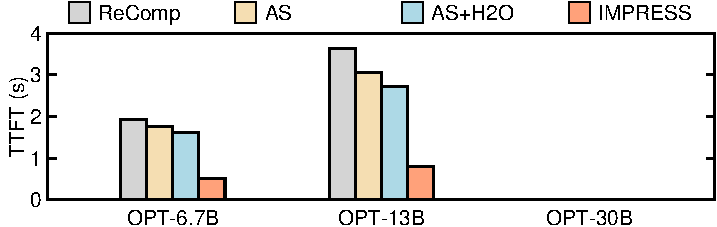
\includegraphics[width=3.3in, height=1in]{ttft_ds1.pdf}
%	}
%	\hspace{0.1in}
%	\subfigure[ds2]{
%		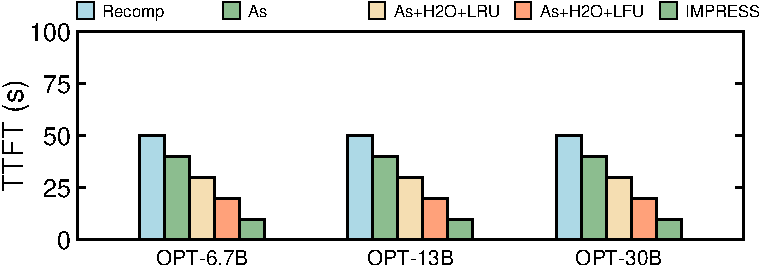
\includegraphics[width=3.3in, height=1in]{ttft_ds2.pdf}
%	}
%	\subfigure[ds3]{
%		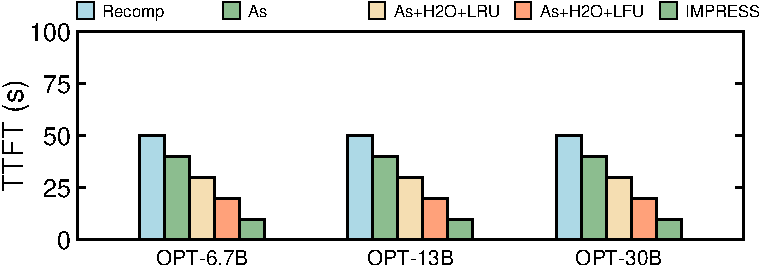
\includegraphics[width=3.3in, height=1in]{ttft_ds3.pdf}
%	}
%	\hspace{0.1in}
%	\subfigure[ds4]{
%		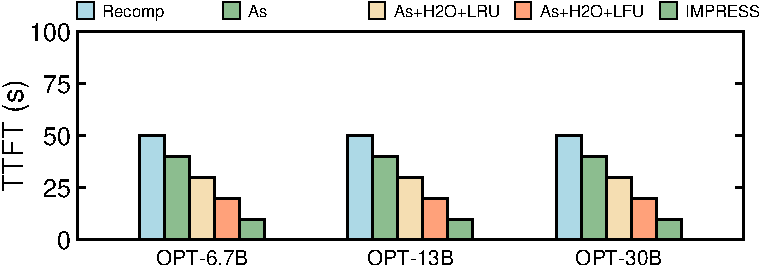
\includegraphics[width=3.3in, height=1in]{ttft_ds4.pdf}
%	}
%	\vspace{-0.1in}
%	\caption{
%		The average TTFT of various systems across four dataset and three models.}
%	\label{fig:overall_ttft}
%\end{figure*}

%\begin{figure*}
%	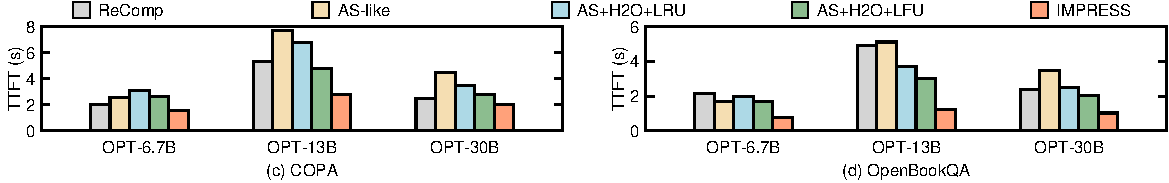
\includegraphics[width=3.4in, height=1.2in]{ttft_ds3_ds4.pdf}
%%	\vskip 1em
%	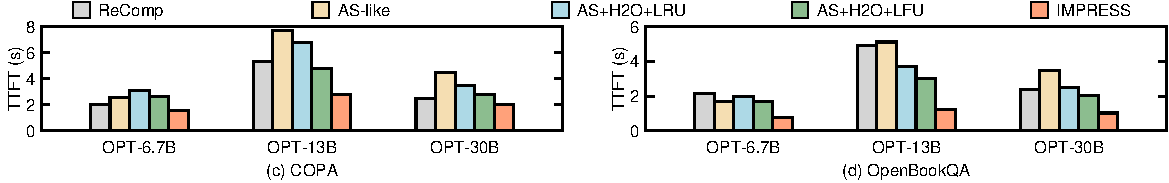
\includegraphics[width=3.4in, height=1.2in]{ttft_ds3_ds4.pdf}
%	\vspace{-0.1in}
%	\caption{
%		The average TTFT of various systems across four dataset and three models.}
%	\label{fig:overall_ttft}
%\end{figure*}


%\begin{figure*}
%	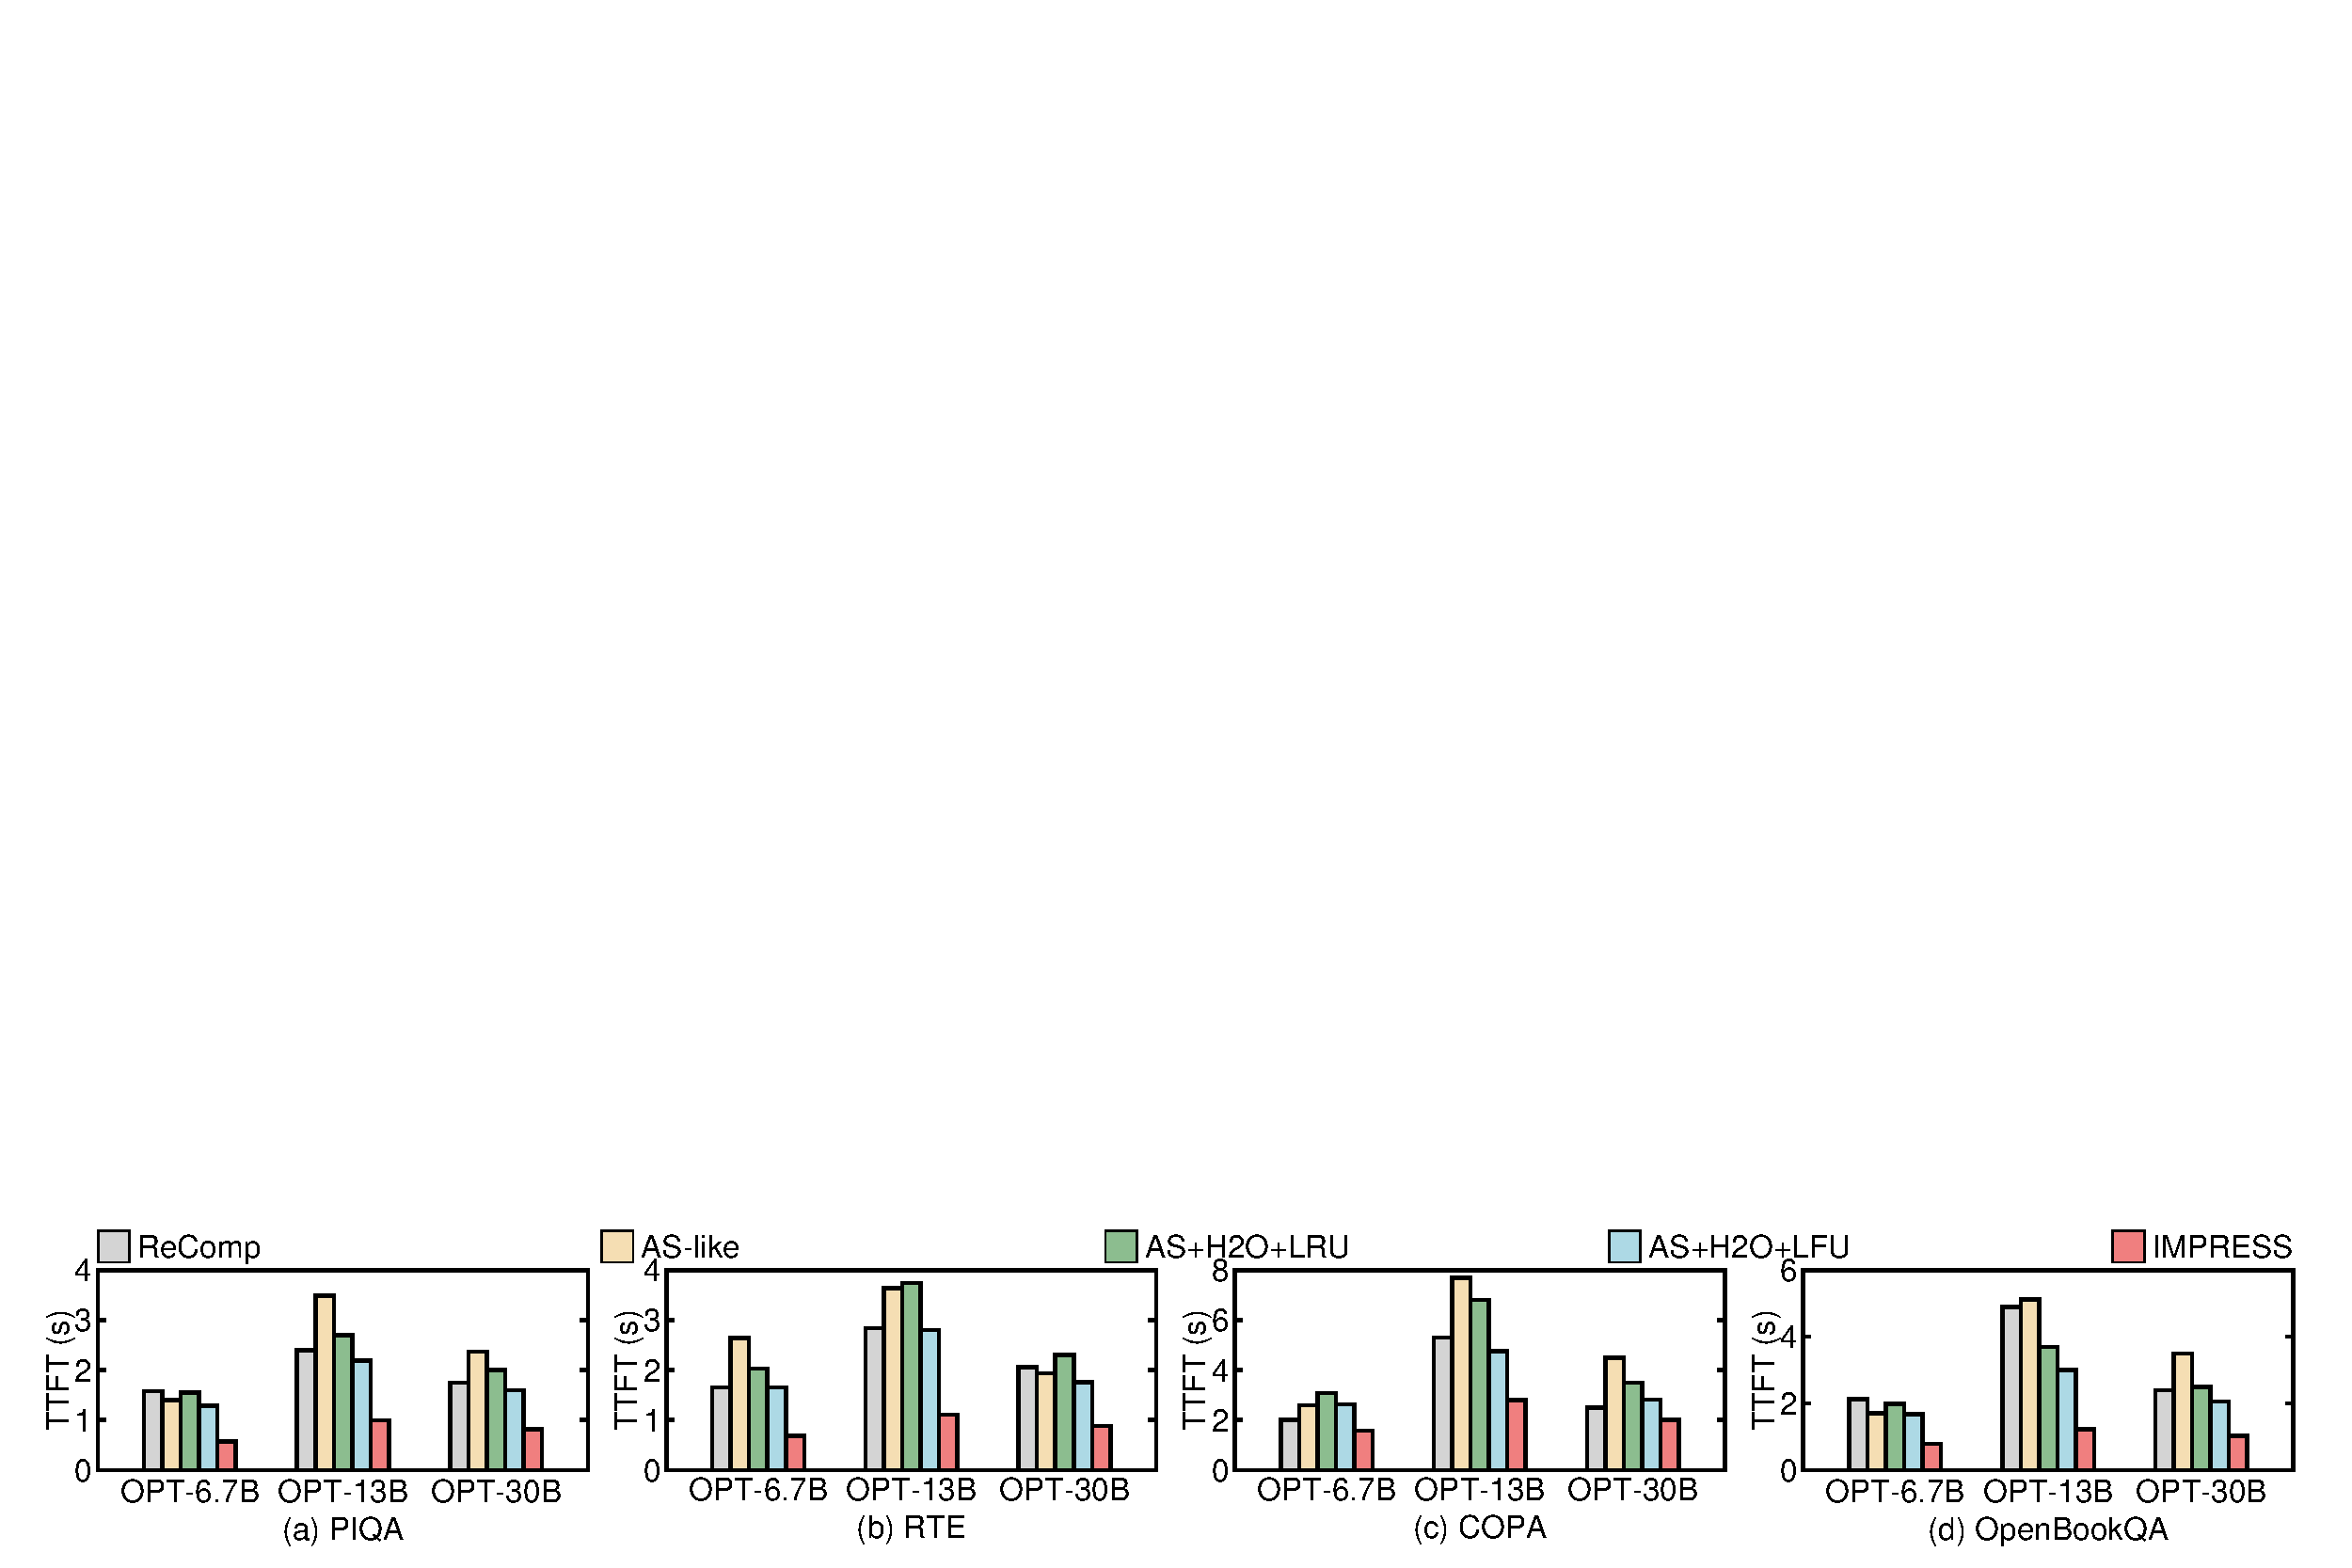
\includegraphics[width=7in, height=1.2in]{ttft_ds1_ds2_ds3_ds4.pdf}
%	\vspace{-0.1in}
%	\caption{
%		The average TTFT of various systems across four dataset and three models.}
%	\label{fig:overall_ttft}
%\end{figure*}

\begin{figure}
	\centering
	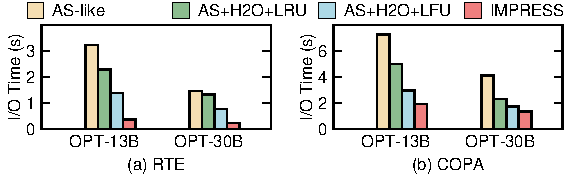
\includegraphics[width=3.3in, height=1in]{iotime.pdf}
	 \vspace{-0.1in}
	\caption{Prefix KV loading time on the RTE dataset.}
	\label{fig:iotime}
	\vspace{-0.1in}
\end{figure}



\subsection{Overall Performance}
\label{exp:overall}

\noindent \textbf{Model generation quality.}
Figure~\ref{fig:overall_acc} illustrates the impact of different systems on model generation quality at various prefix KV retention ratios. 
As ReComp and AS-like share the same accuracy, and AS+H2O+LRU and AS+H2O+LFU also show identical accuracy, we present only the accuracy of ReComp, AS+H2O+LRU, and \pname{} for simplicity.
It shows that \pname{} has a negligible impact on accuracy across these datasets
and models, achieving accuracy drop less than 1\% compared to ReComp or AS+H2O+LRU. In
some cases, \pname{} even slightly improves accuracy over ReComp, suggesting
that focusing on more important tokens can sometimes enhance generation quality.



\noindent \textbf{The average TTFT.}
%We warm up both CPU and GPU caches for all systems, \he{except ReComp}, before evaluating TTFT.
We pre-warm both CPU and GPU caches for all systems, except ReComp (which doesn’t require prefix KV reuse), before evaluating TTFT.
We set the KV retention ratio to 50\% for COPA and 25\% for the other three
datasets across all systems. With this setup, \pname{} shows an average accuracy
reduction of 0.2\% compared to ReComp.
%Figure~\ref{fig:overall_ttft} presents the average TTFT per request with different systems. 
%We have two observations.
%First, \pname{} significantly outperforms alternative systems, with a performance improvement of 1.2$\times$ to 2.8$\times$ over the leading solutions. This advantage stems from \pname{}'s ability to cut the I/O time for loading prefix KVs into GPU memory by 1.5$\times$ to 3.8$\times$, as illustrated in Figure~\ref{fig:iotime}. Conversely, other systems suffer from longer I/O times, occasionally leading to a TTFT that surpasses even ReComp's.
%Second, the performance gains of \pname{} fluctuate across different datasets and models. This variation is attributed to the distinct sizes of prefix KV data and the computational demands of each dataset and model. It's important to note that OPT-30B achieves a shorter TTFT than OPT-13B, as it handles shorter prefixes to prevent GPU memory overflow, which can cause out-of-memory errors.
\fvc{
Figure~\ref{fig:overall_ttft} shows the average TTFT per request for different systems. \pname{} outperforms alternatives, with a 1.2$\times$ to 2.8$\times$ improvement over leading solutions, due to a 1.5$\times$ to 3.8$\times$ reduction in I/O time for loading prefix KVs into GPU memory (Figure~\ref{fig:iotime}). Other systems have longer I/O times, sometimes exceeding ReComp's TTFT. Besides, \pname{}'s performance gains vary across datasets and models due to different prefix KV sizes and computational demands. Notably, OPT-30B has a shorter TTFT than OPT-13B, as it uses shorter prefixes to avoid GPU memory overflow.
}


\noindent 
\fv{
\textbf{The tail latency.} \pname{} achieves the shortest p99 tail TTFT. For example, on the RTE dataset with OPT-30B model, the p99 latencies for ReComp, AS-like, AS+H2O+LRU, AS+H2O+LFU, and \pname{} are 3.9s, 9.3s, 6.6s, 5.9s, and 2.95s, respectively. This shows \pname{} effectively reduces the tail I/O latency when KVs are loaded from SSD.
}

\begin{figure}
	\centering
	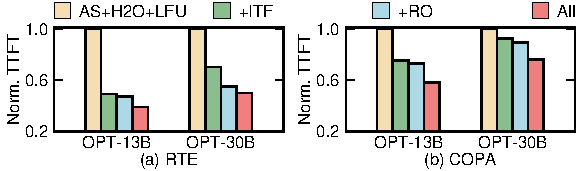
\includegraphics[width=3.3in, height=1in]{indiv_ds1_ds2.pdf}
	\vspace{-0.1in}
	\caption{The performance impact of each optimization.}
	\label{fig:indiv}
	\vspace{-0.1in}
\end{figure}
